\section{Hypertranscendence of the conjugacy}
\label{a:sec:ht}

This section makes the obstruction to an elementary closed form precise, and
delimits exactly what it does and does not assert. The logical skeleton is short:
(i) every elementary function satisfies an algebraic differential equation;
(ii) differential algebraicity survives compositional inversion;
(iii) by a theorem of Becker and Bergweiler, a solution of Schr\"oder's equation
for a rational map of degree at least two can be differentially algebraic only
when the underlying fixed point is \emph{repelling};
(iv) for $r\in(0,1)$ the fixed point $0$ of $f_r$ is attracting.
Hypertranscendence of $\psi_r$ for every subcritical parameter follows at once ---
with no exceptional cases to exclude, because the attracting window contains no
candidates at all. We then explain, with equal care, why this theorem does
\emph{not} by itself settle the status of the individual numbers $A(p_0)$ or of
the map $p\mapsto A(p)$, and we record the numerical evidence bearing on those.

\subsection{Differential algebraicity, hypertranscendence, elementarity}
\label{a:sec:definitions}

\begin{definition}[Differentially algebraic; hypertranscendental]
\label{a:def:da}
A function $g$, holomorphic on a domain (or a formal power series), is
\emph{differentially algebraic over $\mathbb{C}(z)$} if there exists a non-zero
polynomial $P$ in $n+2$ variables, for some $n\ge0$, with
\begin{equation*}
P\bigl(z,\,g(z),\,g'(z),\,\dots,\,g^{(n)}(z)\bigr)\equiv 0 .
\end{equation*}
Otherwise $g$ is \emph{differentially transcendental}, or
\emph{hypertranscendental}.
\end{definition}

Two closure facts make this the right notion for the present purpose.

\begin{lemma}[Elementary $\Rightarrow$ differentially algebraic]
\label{a:lem:elemDA}
Every elementary function in the Liouville sense --- any function reachable from
$\mathbb{C}(z)$ by a finite tower of algebraic operations, exponentials and
logarithms --- is differentially algebraic. Consequently a hypertranscendental
function is not elementary.
\end{lemma}

\begin{proof}[Proof sketch]
Each storey of a Liouvillian tower preserves differential algebraicity: algebraic
extensions do so by elimination; if $g$ is differentially algebraic then so are
$\ee^{g}$ and $\ln g$, their defining first-order relations combining with the
equation for $g$; and the class is closed under field operations and composition.
These closure properties are classical; see Rubel's survey \cite{Rubel1989}.
\end{proof}

\begin{lemma}[Closure under compositional inversion]
\label{a:lem:invDA}
Let $g$ be holomorphic near $0$ with $g(0)=0$ and $g'(0)\neq0$, and let $g^{-1}$
denote its local compositional inverse. Then $g$ is differentially algebraic over
$\mathbb{C}(z)$ if and only if $g^{-1}$ is
\cite{Moore1896,BoshernitzanRubel1986}.
\end{lemma}

\Cref{a:lem:invDA} matters because the literature states Schr\"oder-equation
results in two equivalent but opposite conventions, and conflating them is an easy
way to misquote a theorem. Our $\psi_r$ is the \emph{linearising coordinate}:
$\psi_r(f_r(z))=r\,\psi_r(z)$. The function classified by Becker and Bergweiler
(and by Ritt before them) is the \emph{linearising parametrisation}
$\varphi_r=\psi_r^{-1}$, which satisfies
\begin{equation}
\label{a:eq:schroderparam}
\varphi_r(r\,t)=f_r\bigl(\varphi_r(t)\bigr),
\qquad
\varphi_r(0)=0,\quad \varphi_r'(0)=1 .
\end{equation}
By \cref{a:lem:invDA}, hypertranscendence of either function transfers to the
other.

\subsection{The Becker--Bergweiler theorem, stated precisely}
\label{a:sec:BB}

The result needed here is the 1995 classification of differentially algebraic
Schr\"oder functions \cite{Becker1995}, quoted in the form given in Fernandes'
survey of the Schr\"oder, B\"ottcher and Abel equations \cite[Thm~3.1]{Fernandes2021}.

\begin{theorem}[Becker--Bergweiler \cite{Becker1995}; as restated in {\cite[Thm~3.1]{Fernandes2021}}]
\label{a:thm:BB}
Let $R$ be a rational map of degree at least two with $R(0)=0$ and multiplier
$s=R'(0)$, where $s\neq0$ and $s$ is not a root of unity (for $|s|=1$ the
Schr\"oder function is understood as a formal series). Let $\varphi$, normalised
by $\varphi(0)=0$ and $\varphi'(0)=1$, solve $\varphi(st)=R(\varphi(t))$. If
$\varphi$ is differentially algebraic over $\mathbb{C}(t)$, then:
\begin{enumerate}[label=\textup{(\roman*)}]
\item the fixed point $0$ is \emph{repelling}, $|s|>1$; and
\item $\varphi$ is a M\"obius transformation of one of
\begin{equation*}
\exp(\alpha t^{\rho}),
\qquad
\cos(\alpha t^{\rho}+\beta),
\qquad
\wp(\alpha t^{\rho}+\beta),\ \wp^{2},\ \wp^{3},\ \wp'(\alpha t^{\rho}+\beta),
\end{equation*}
where $\wp$ is a Weierstrass function, $\rho\in\mathbb{Q}$ is such that the
function concerned is meromorphic on $\mathbb{C}$, $\alpha\neq0$, and $\beta$ is a
fraction of a period. Correspondingly $R$ is M\"obius-conjugate to $z^{\pm d}$, to
$\pm T_d$ (Chebyshev), or to a Latt\`es map.
\end{enumerate}
\end{theorem}

\begin{remark}[Lineage and independent corroboration]
\label{a:rem:lineage}
For $|s|>1$ --- the Poincar\'e-function case --- the classification goes back to
Ritt in 1926 \cite{Ritt1926}; Becker and Bergweiler completed the picture for the
three classical functional equations at once, and Bergweiler's later account with
Aschenbrenner \cite{AschenbrennerBergweiler2015} assigns the exceptional list
explicitly to the repelling case. Di~Vizio and Fernandes
\cite{DiVizioFernandes2021} have given an independent difference-Galois proof of
Ritt's theorem; notably, their Theorems~1.2 and~4.2 assume only that $s$ is
neither zero nor a root of unity --- no condition $|s|>1$ --- and show that any
differentially algebraic solution of $y(R(x))=s\,y(x)$ (our $\psi$-convention,
with no inversion needed) must already satisfy a first-order equation of Ritt type
$(y')^{\rho}=B(x)\,y^{\,j}$. The structure underlying \cref{a:thm:BB} therefore
does not hang on a single paper.
\end{remark}

\subsection{Hypertranscendence throughout the subcritical window}
\label{a:sec:mainht}

\begin{theorem}[No exceptional parameters in $(0,1)$]
\label{a:thm:mainht}
For every $r\in(0,1)$, the Koenigs function $\psi_r$ of $f_r(z)=rz(1-z)$ at $0$
is hypertranscendental over $\mathbb{C}(z)$: it satisfies no algebraic
differential equation. In particular, $\psi_r$ is not an elementary function.
\end{theorem}

\begin{proof}
Fix $r\in(0,1)$. The map $f_r$ is rational of degree two, fixes $0$, and its
multiplier $s=f_r'(0)=r$ satisfies $0<s<1$; the hypotheses of \cref{a:thm:BB}
hold, with $0$ attracting. Suppose, for contradiction, that $\psi_r$ were
differentially algebraic. Its local inverse $\varphi_r=\psi_r^{-1}$ solves the
parametrisation form \cref{a:eq:schroderparam} with the stated normalisation, and
by \cref{a:lem:invDA} it would be differentially algebraic too.
\Cref{a:thm:BB}(i) would then force $|r|>1$, contradicting $r\in(0,1)$. Hence
$\psi_r$ is hypertranscendental, and non-elementarity follows from
\cref{a:lem:elemDA}.
\end{proof}

\begin{remark}[The exceptional set inside the window is empty, not merely avoided]
\label{a:rem:empty}
An earlier form of this argument reasoned through the parameter plane: the affine
conjugacy $c(r)=(2r-r^{2})/4$ of \cref{a:lem:affine} sends $r\in(0,1)$ to
$c\in(0,\tfrac14)$, which avoids the exceptional quadratic parameters $c=0$
(reached at $r=2$) and $c=-2$ (reached at $r=4$, and also at $r=-2$). That
observation is true but logically superfluous, and it invites a question it cannot
answer --- \emph{is the exceptional list, restricted to the window, complete?} The
route through \cref{a:thm:BB}(i) dissolves the question: the exceptional
Schr\"oder functions exist only over \emph{repelling} fixed points, so the
attracting window contains no candidates whatsoever, and no enumeration of
exceptional parameters is required. Consistently, the classical elementary cases
of \cref{a:app:integrable} have multipliers $2$ and $4$ at the linearised fixed
point --- both repelling: they are Poincar\'e-type linearisations, and neither can
be pressed into service for $r\in(0,1)$.
\end{remark}

\begin{figure}[H]
\centering
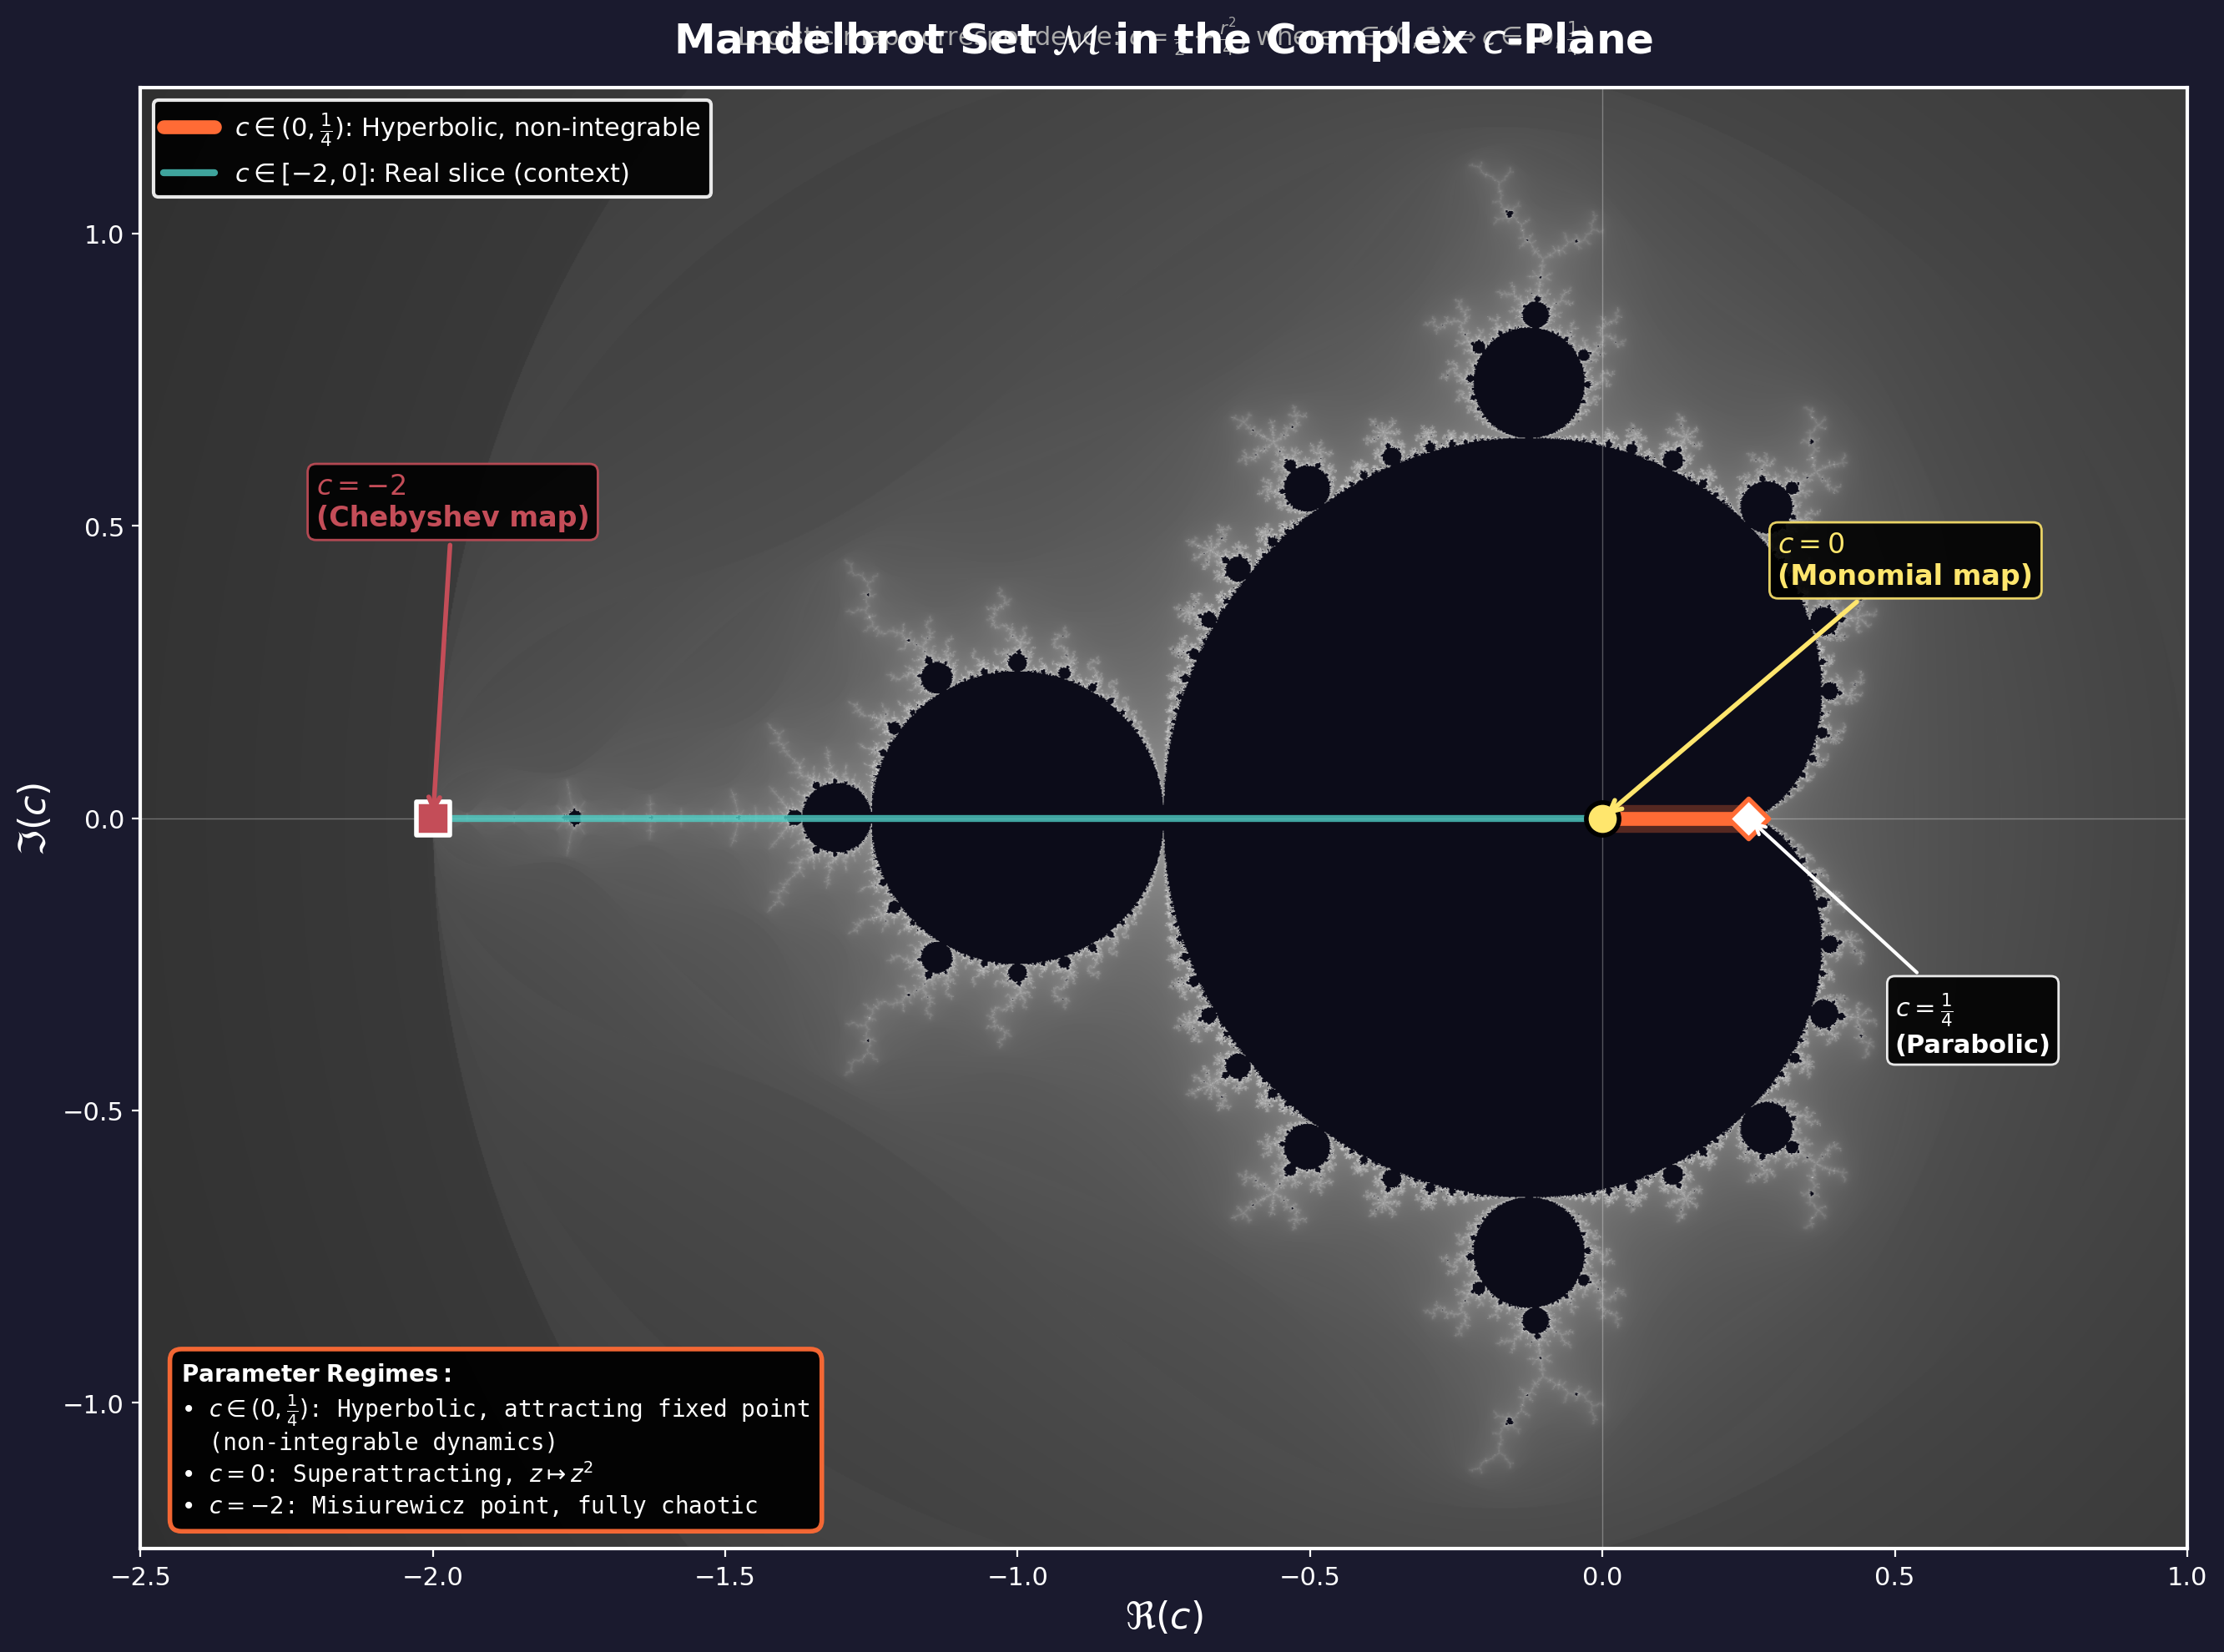
\includegraphics[width=0.72\textwidth]{figures/figure4_mandelbrot_context.png}
\caption{The Mandelbrot set in the complex $c$-plane, with the interval
$c\in(0,\tfrac14)$ highlighted. Under the correspondence $c=(2r-r^2)/4$ of
\cref{a:eq:cofr} this is the image of the subcritical branching window
$r=2p\in(0,1)$, and it forms the real diameter of the main cardioid, running from
the centre $c=0$ to the parabolic cusp $c=\tfrac14$, which is criticality. The two
integrable parameters are marked: $c=0$ (monomial, reached in logistic coordinates
at $r=2$) and $c=-2$ (Chebyshev, $r=4$), the latter at the far tip of the real
slice. In the light of \cref{a:rem:empty} this picture is a consistency check on
the theorem rather than part of the proof: the exceptional linearisations live
over repelling fixed points, which the attracting window excludes outright. Note
that $c(r) = c(2-r)$, so each $c\in(0,\tfrac14)$ is the image of two logistic
parameters, $r$ and $2-r$; these correspond to the two fixed points of $z^2+c$,
with multipliers $r$ and $2-r$, and it is the attracting one, $r<1$, that governs
$A(p)$.}
\label{a:fig:mandelbrot}
\end{figure}

\begin{remark}[Germ versus basin]
\label{a:rem:basin}
\Cref{a:thm:mainht} concerns $\psi_r$ as an analytic function; the quantity
$A(p)=2\Psi_r(\tfrac12)$ of \cref{a:eq:AeqKoenigs} uses its extension to the real
basin of attraction, since for $p\ge\tfrac13$ the point $\tfrac12$ lies outside
the disc on which Koenigs' series is guaranteed to converge (radius $(1-r)/r$).
The extension is by finitely many applications of the functional equation,
\begin{equation*}
\Psi_r(w)=r^{-N}\,\psi_r\bigl(f_r^{\circ N}(w)\bigr)
\quad\text{for $N$ large enough that $f_r^{\circ N}(w)$ enters the germ,}
\end{equation*}
and an algebraic differential equation, if one held on any subdomain, would
persist under this analytic continuation. Hypertranscendence of the germ and of
the basin extension are therefore equivalent statements, and the identity
\cref{a:eq:AeqKoenigs} is unaffected.
\end{remark}

\begin{figure}[H]
\centering
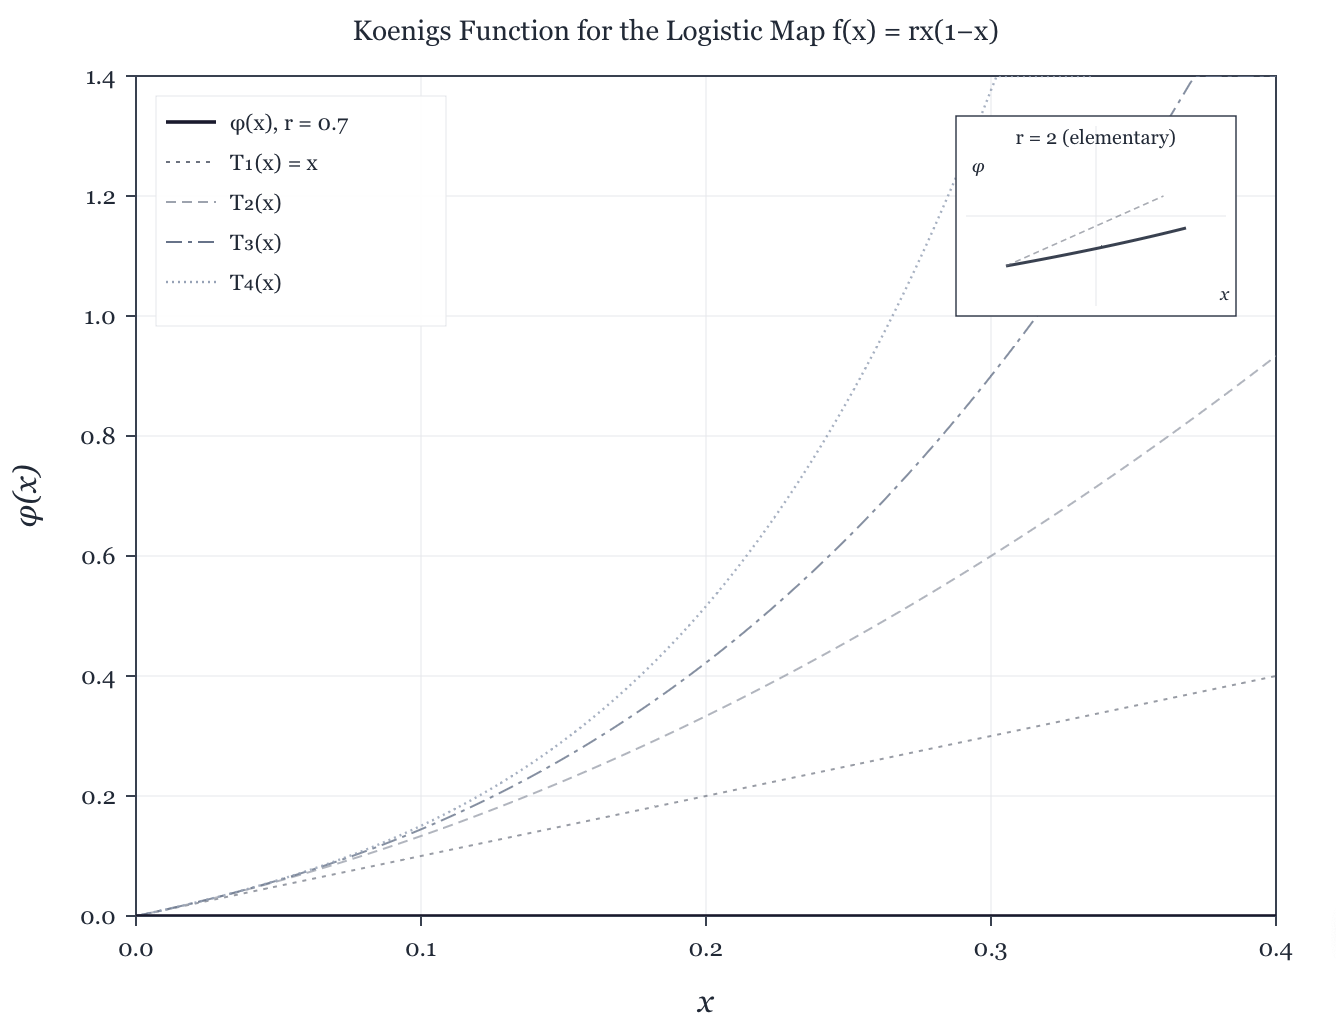
\includegraphics[width=0.72\textwidth]{figures/figure3_numerical_koenigs.png}
\caption{Numerical approximation of a Koenigs function for a logistic multiplier
in $(0,1)$, with low-order Taylor polynomials near the origin. Elementary closed
forms exist only for exceptional multipliers outside this range
(\cref{a:app:integrable}).}
\label{a:fig:numkoenigs}
\end{figure}

\begin{figure}[ht]
\centering
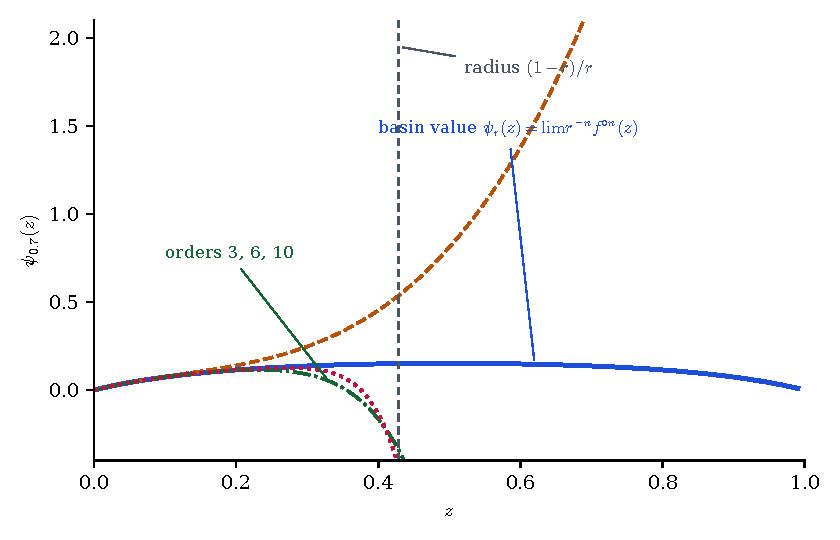
\includegraphics[width=0.86\textwidth]{figures/koenigs_domain.pdf}
\caption{Germ versus basin for the Koenigs function at $r=0.7$. The solid curve
is the basin value $\psi_r(z)=\lim_n r^{-n}f_r^{\circ n}(z)$, computed by direct
orbit iteration and smooth on the whole of $[0,1)$; the dashed curves are Taylor
partial sums of orders $3$, $6$ and $10$ about the origin, obtained by iterating
the functional equation $\psi_r\circ f_r = r\psi_r$ on truncated series. The
truncations agree with the basin value inside the guaranteed disc of radius
$(1-r)/r$ (vertical line) and diverge beyond it, the higher orders first ---
exactly the germ/basin distinction of \cref{a:rem:basin}. Evaluating
$A(p)=2\Psi_r(\tfrac12)$ therefore requires the basin extension whenever
$\tfrac12$ lies outside the disc, that is for $p\ge\tfrac13$.}
\label{a:fig:koenigsdomain}
\end{figure}
